\section{Results}
\label{sec:results}

In this section, we present the main results of our model training and inference. We present the results of supervised pretraining in section \ref{sec:supervised results}, and the results of the reinforcement learning in section \ref{sec:rl results}. Finally, we experiment with the final model's ability to generate puzzles in section \ref{sec:final tests}.


\subsection{Supervised results}
\label{sec:supervised results}

After training our model with the setup described in section \ref{sec:supervised training}, we obtain the loss curve shown in Figure \ref{fig:training_loss}. We see that clearly the model learns the data, as the test loss decreases. At around 1,000,000 training steps, however, we observe that the model starts to overfit slightly, as the test loss starts to increase once again. We store checkpoints of our model at intervals of 100,000 steps, and therefore, we choose the model trained for 1,000,000 steps. During some training runs, we observed instability and model collapse, however, we managed to solve this by incorporating clipping to the weights in the evidence lower bound \eqref{eq:ELBO} as done by \citeauthor{shi2025simplifiedgeneralizedmaskeddiffusion}. In the latest training run, we observed no instability. Comparing Figure \ref{fig:training_loss} to Figure \ref{fig:supervised_training_metrics}, we observe that the loss corresponds quite well with the real metrics we are interested in.

\textcolor{red}{TODO: Write a paragraph analyzing the loss curve. Some suggestions on what to include:
\begin{itemize}
    \item \textbf{Overall trend:} Describe the initial rapid decrease in the negative evidence lower bound and the subsequent plateau.
    \item \textbf{Overfitting point:} Explicitly point out the divergence at 1,000,000 steps mentioned in the caption, where overfitting begins (e.g. validation loss increasing or plateauing while training loss decreases).
    \item \textbf{Checkpoint selection:} State which checkpoint was ultimately chosen for the next phases (e.g. early stopping right before 1M steps) based on this curve.
    \item \textbf{Stability:} Mention if the training was stable or if there were any notable spikes/anomalies in the loss.
    \item \textbf{Connection to performance:} Briefly relate how the loss stabilization corresponds to the model learning the basic rules of chess (which might explain the rapid initial drop).
\end{itemize}}
\begin{figure}[h]
    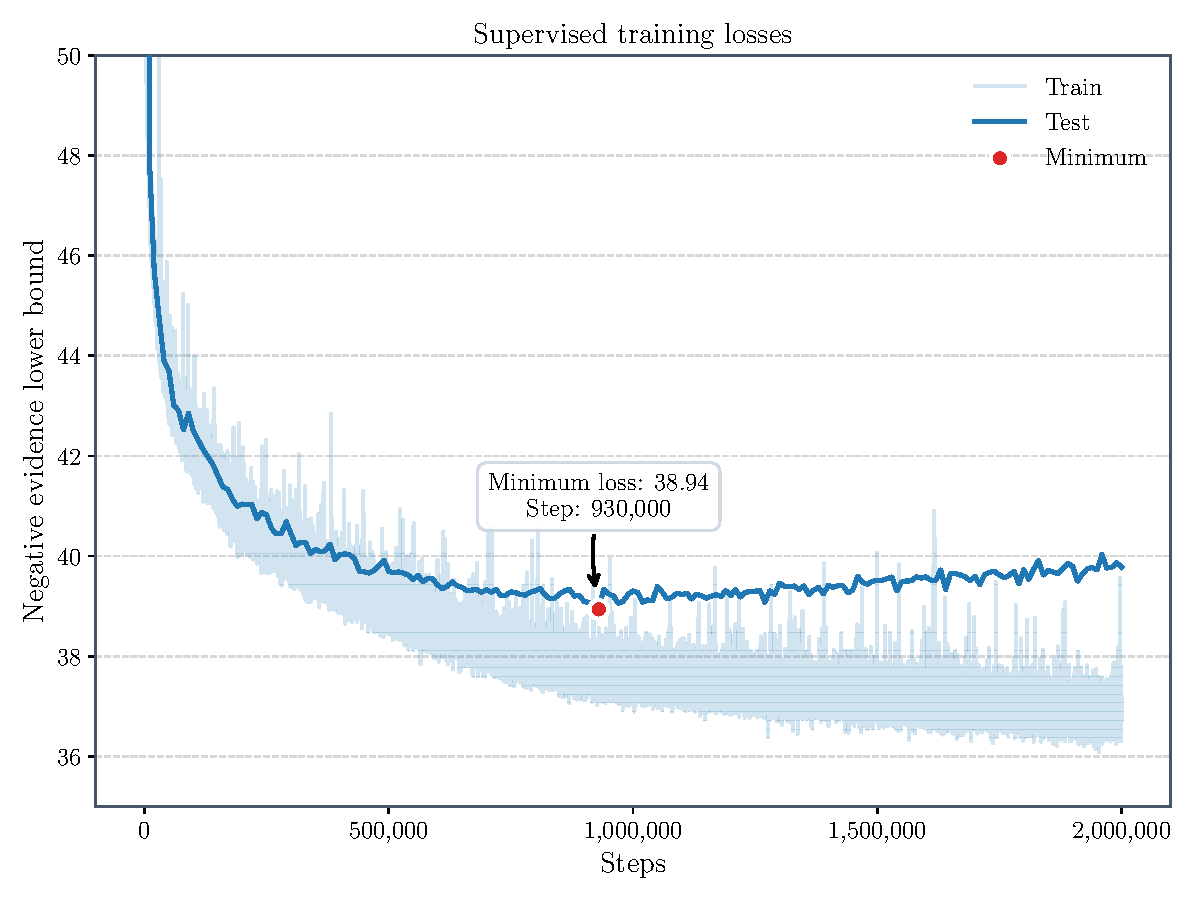
\includegraphics[width=\textwidth]{./sections/figures/supervised_training_progress/Training_loss.pdf}
    \caption{The negative evidence lower bound as a function of the training steps. After around 1,000,000, we observe clear overfitting.}
    \label{fig:training_loss}
\end{figure}

As described in section \ref{sec:evaluation criteria}, our main evaluation metric is the proportion of positions that pass both the uniqueness and the counter-intuitiveness criteria, i.e. the puzzle rate. Additionally, we monitor the legal rate, the uniqueness rate and the counter intuitiveness rate individually, as well as some diversity filtering metrics. In figure \ref{fig:supervised_training_metrics}, we see the evolution of these metrics over the supervised training run. Each data point is collected by sampling 10,000 positions from the model for each checkpoint, which are stored on 100,000-step intervals. We notice that the legal rate quickly improves to the final value, whereas the other metrics, which are more nuanced, take longer to improve. We see that the uniqueness rate steadily improves, however, the counter intuitiveness values and consequently the puzzle rate are quite noisy. This is due to the high variance of the counter-intuitiveness metric, which stems from Stockfish being great at finding the correct solutions very quickly.

In figure \ref{fig:supervised_training_metrics}, we see that the values of the different metrics increase over the training steps. \textcolor{red}{Talk about overfitting (context from test probably decreases somewhere)}

% \ref{sec:supervised training}


\begin{figure}[htbp]
    \centering
    
\includegraphics[width=0.49\linewidth]{sections/figures/supervised_training_progress/Legal_rate.pdf}
    \hfill
    
\includegraphics[width=0.49\linewidth]{sections/figures/supervised_training_progress/Uniqueness_rate.pdf}
    
    \vspace{0.5cm}
    
    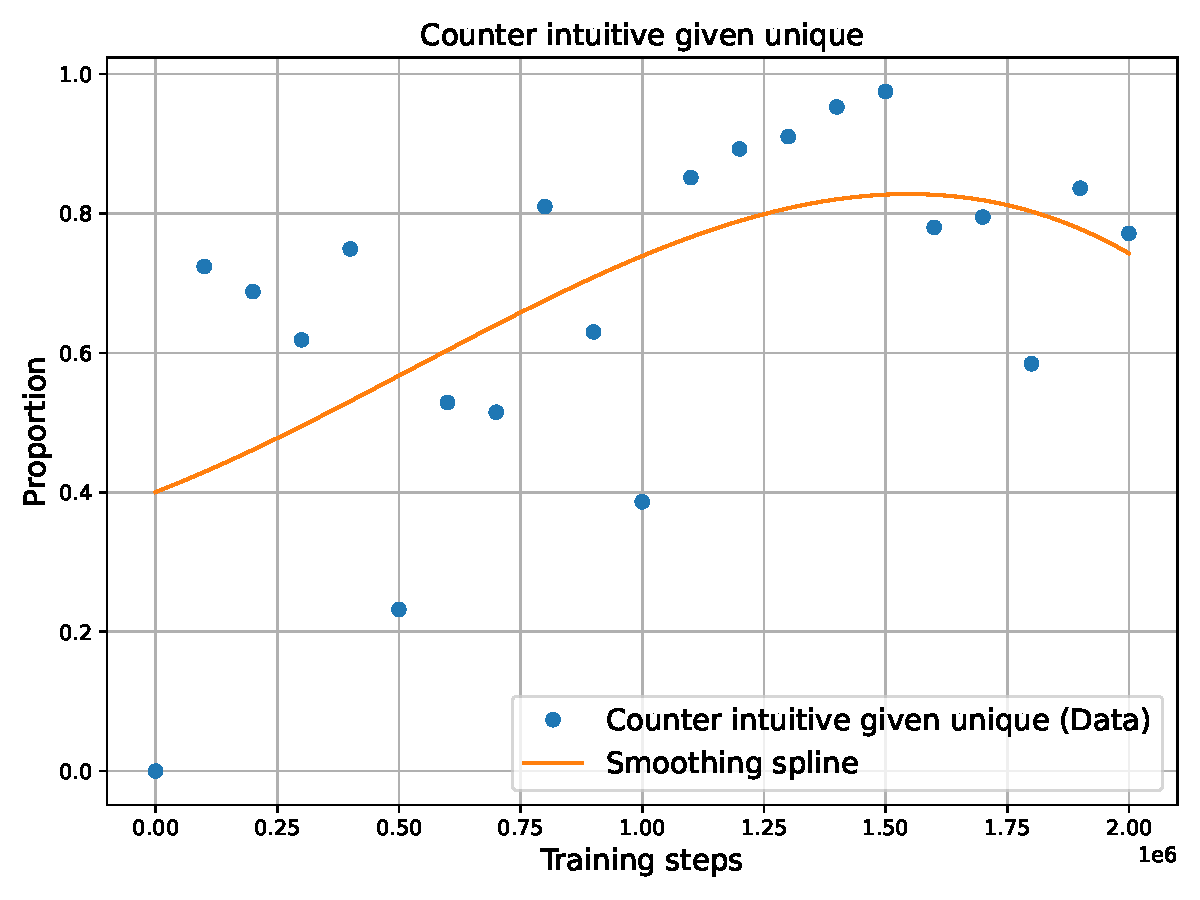
\includegraphics[width=0.49\linewidth]{sections/figures/supervised_training_progress/Counter_intuitive_given_unique.pdf}
    \hfill
    
\includegraphics[width=0.49\linewidth]{sections/figures/supervised_training_progress/Puzzle_rate.pdf}
    \caption{Evolution of the primary quality metrics with context from the training set during supervised pretraining.}
    \label{fig:supervised_training_metrics}
\end{figure}


\subsection{Reinforcement learning results}
\label{sec:rl results}





\subsection{Tests with the final model}
\label{sec:final tests}

\textcolor{red}{Example positions etc.}

